\documentclass{article}
\usepackage{graphicx}
\usepackage[margin=1.5cm]{geometry}
\usepackage{amsmath}

\begin{document}

\title{Monday Reading Assessment: Unit 4, Forces}
\author{Prof. Jordan C. Hanson}

\maketitle

\section{Memory Bank}

\begin{itemize}
\item Newton's First Law: If $\vec{F}_{net} = 0$, then $\Delta\vec{v}$ = 0.  (An object at rest stays at rest, or an object in motion stays in motion, unless the object has a net external force acting upon it).
\item Newton's Second Law: $\vec{F}_{net} = m\vec{a}$. (The net external force on an object is equal to the mass of the object times the acceleration of the object).
\item Newton's Third Law: $\vec{F}_{AB} = -\vec{F}_{BA}$. (For every action there is an equal and opposite reaction).
\end{itemize}

\section{Chapter 4 - Forces, Continued}

\begin{enumerate}
\item In Fig. \ref{fig:elev}, a man with mass $m$ stands on a bathroom scale in an elevator.  Which of the followinng is true, if the elevator is accelerating upwards?
\begin{itemize}
\item A: The scale reading gives a weight that is larger than $mg$.
\item B: The scale reading gives a weight that is smaller than $mg$.
\item C: The scale reading gives a weight equal to $mg$.
\item D: The scale reading gives a weight of zero.
\end{itemize}
\item 
\begin{figure}[hb]
\centering
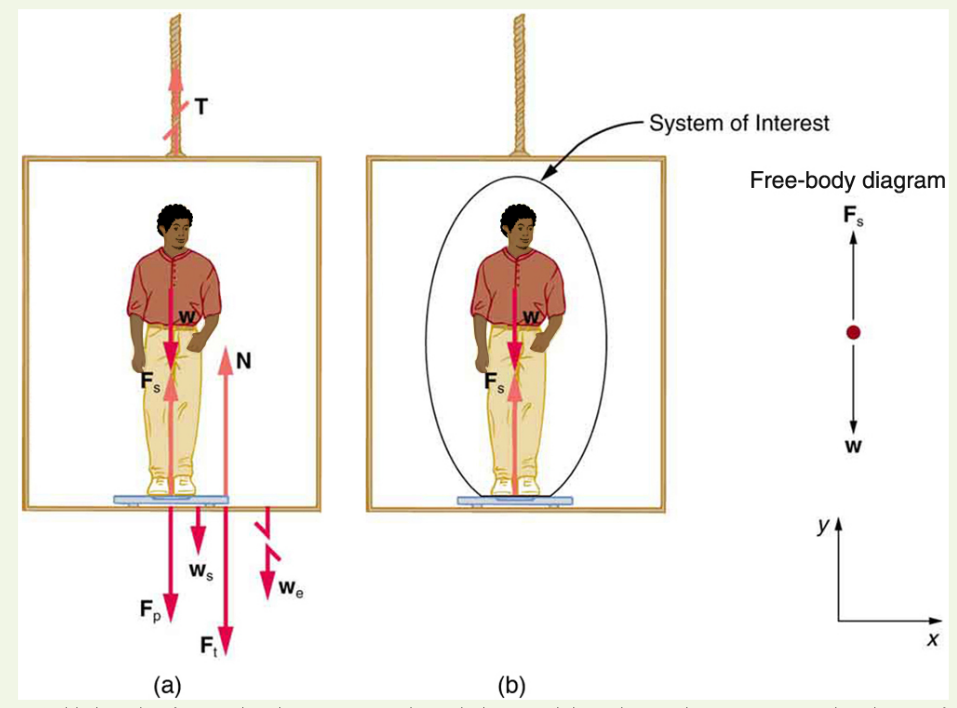
\includegraphics[width=0.35\textwidth]{elevator.png}
\caption{\label{fig:elev} A person of weight $\vec{w}$ stands on a scale in an elevator.}
\end{figure}
In Fig. \ref{fig:elev}, a 75.0-kg man stands on a bathroom scale in an elevator. Calculate what weight does the scale read if: (a) the acceleration of the elevator is +1.0 m/s$^2$, (b) the acceleration of the elevator is -1.0 m/s$^2$, (c) the elevator moves upward at 3.0 m/s, and (d) if the elevator is stationary.
\end{enumerate}

\end{document}
